
\documentclass[11pt,a4paper]{article}

\usepackage[T1]{fontenc}
\usepackage[utf8]{inputenc}
\usepackage{lmodern}
\usepackage[margin=1in]{geometry}
\usepackage{amsmath,amssymb,amsthm,mathtools}
\usepackage{booktabs}
\usepackage{array}
\usepackage{tabularx}
\usepackage{microtype}
\usepackage{enumitem}
\usepackage[hidelinks]{hyperref}
\usepackage[nameinlink,noabbrev]{cleveref}
\usepackage{siunitx}
\usepackage{xcolor}
\usepackage{tcolorbox}
\tcbuselibrary{skins,breakable}
\usepackage{tikz}
\usetikzlibrary{arrows.meta,positioning,calc,fit,backgrounds,decorations.pathmorphing,angles,quotes}
\usepackage{pgfplots}
\pgfplotsset{compat=1.18}
\usepgfplotslibrary{fillbetween}

\setlength{\parskip}{0.45em}
\setlength{\parindent}{0pt}

\newtheorem{theorem}{Theorem}[section]
\newtheorem{proposition}[theorem]{Proposition}
\newtheorem{corollary}[theorem]{Corollary}
\theoremstyle{definition}
\newtheorem{definition}[theorem]{Definition}
\theoremstyle{remark}
\newtheorem*{remark}{Remark}

\DeclareMathOperator{\tr}{Tr}
\DeclareMathOperator{\im}{Im}
\DeclareMathOperator{\re}{Re}

\newcolumntype{Y}{>{\raggedright\arraybackslash}X}

\newcommand{\Seam}{\Sigma}
\newcommand{\inv}{\iota}
\newcommand{\cthree}{c_3}
\newcommand{\bone}{b_1}
\newcommand{\phibase}{\varphi_{\mathrm{base}}}
\newcommand{\phiseam}{\varphi_{\Sigma}}
\newcommand{\phiz}{\varphi_{0}^{\mathrm{ret}}}
\newcommand{\deltatop}{\delta_{\mathrm{top}}}
\newcommand{\gammaY}{\gamma}
\newcommand{\SM}{\mathrm{SM}}
\newcommand{\BR}{\mathrm{BR}}

\numberwithin{equation}{section}

\title{\textbf{TFPT and the Rare Kaon Sector}\\[4pt]\large TFPT-fixed CKM branching ratios
for $K\to\pi\nu\bar\nu$ with standard short-distance input}
\author{Stefan Hamann \and Alessandro Rizzo}
\date{\today}

\begin{document}
\maketitle

\begin{abstract}
The TFPT minimal kernel fixes the CKM matrix entirely through the carrier seed
$\phiz$ and the $\mathbb Z_6$ transport grammar, without fitting to flavor data.
This note traces the resulting prediction chain for the rare
kaon decays $K^+\to\pi^+\nu\bar\nu$ and $K_L\to\pi^0\nu\bar\nu$,
using the exact PDG-convention CKM matrix built from the TFPT mixing
angles and CP phase, combined with modern short-distance input.
The TFPT-fixed branching ratios are
\[
\BR(K^+\to\pi^+\nu\bar\nu)=\num{9.40e-11},
\qquad
\BR(K_L\to\pi^0\nu\bar\nu)=\num{3.47e-11},
\]
with a sharp operational test corridor: a stable NA62 result outside
$[7,12]\times 10^{-11}$ for the charged channel, or a KOTO result
incompatible with the Grossman--Nir correlation, would break the
present TFPT flavor bridge. The current NA62 observation
$\BR(K^+)=(13.0^{+3.3}_{-3.0})\times 10^{-11}$ is consistent with
the prediction at the $1\sigma$ level.
\end{abstract}

\tableofcontents

\bigskip

\begin{figure}[ht]
\centering
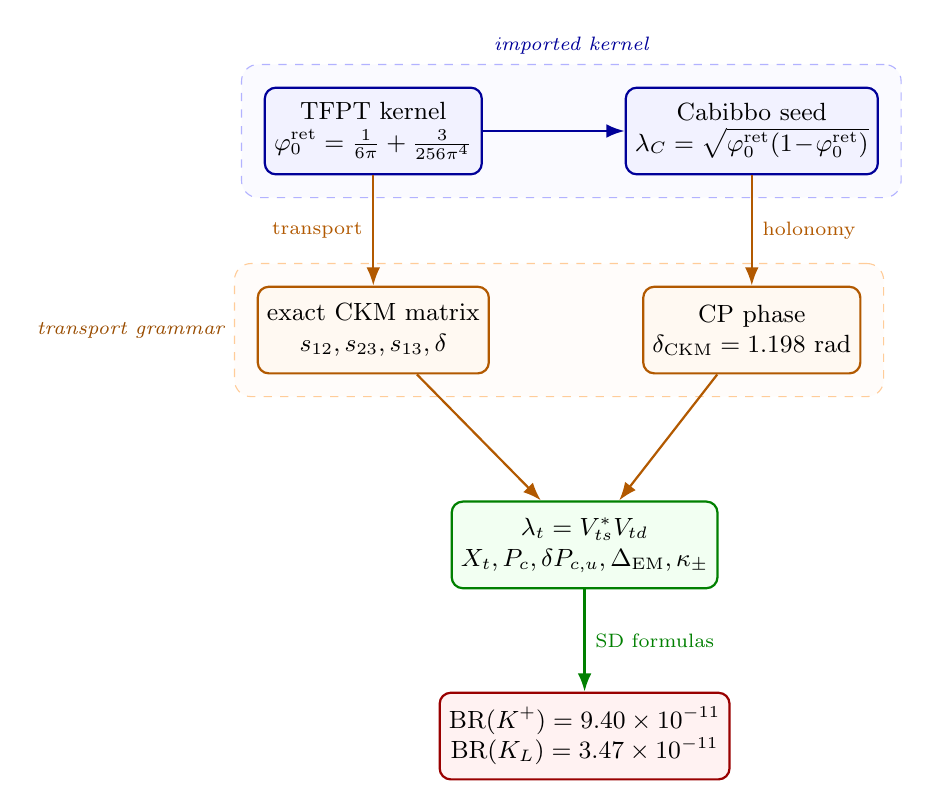
\begin{tikzpicture}[
    >=Latex,
    kernel/.style={draw=blue!60!black, thick, rounded corners=4pt,
        fill=blue!5, align=center, minimum width=2.6cm, minimum height=1.1cm,
        font=\small},
    transport/.style={draw=orange!70!black, thick, rounded corners=4pt,
        fill=orange!5, align=center, minimum width=2.6cm, minimum height=1.1cm,
        font=\small},
    sector/.style={draw=green!50!black, thick, rounded corners=4pt,
        fill=green!5, align=center, minimum width=2.7cm, minimum height=1.1cm,
        font=\small},
    result/.style={draw=red!60!black, thick, rounded corners=4pt,
        fill=red!5, align=center, minimum width=2.6cm, minimum height=1.1cm,
        font=\small\bfseries},
    arrlabel/.style={font=\scriptsize, fill=white, inner sep=1.5pt},
]
\node[kernel] (seed) {TFPT kernel\\$\phiz=\frac{1}{6\pi}+\frac{3}{256\pi^4}$};
\node[kernel, right=1.8cm of seed] (cabibbo) {Cabibbo seed\\$\lambda_C=\sqrt{\phiz(1\!-\!\phiz)}$};
\node[transport, below=1.4cm of seed] (ckm) {exact CKM matrix\\$s_{12},s_{23},s_{13},\delta$};
\node[transport, below=1.4cm of cabibbo] (phase) {CP phase\\$\delta_{\mathrm{CKM}}=1.198$ rad};
\node[sector, below right=1.6cm and -0.5cm of ckm] (lambda)
    {$\lambda_t=V_{ts}^*V_{td}$\\$X_t,P_c,\delta P_{c,u},\Delta_{\mathrm{EM}},\kappa_{\pm}$};
\node[result, below=1.3cm of lambda] (br) {$\BR(K^+)=9.40\times10^{-11}$\\$\BR(K_L)=3.47\times10^{-11}$};

\draw[->, thick, blue!60!black] (seed) -- (cabibbo);
\draw[->, thick, orange!70!black] (seed) -- (ckm)
    node[arrlabel, midway, left=2pt]{transport};
\draw[->, thick, orange!70!black] (cabibbo) -- (phase)
    node[arrlabel, midway, right=2pt]{holonomy};
\draw[->, thick, orange!70!black] (ckm) -- (lambda);
\draw[->, thick, orange!70!black] (phase) -- (lambda);
\draw[->, thick, green!50!black] (lambda) -- (br)
    node[arrlabel, midway, right=2pt]{SD formulas};

\begin{scope}[on background layer]
    \node[draw=blue!30, dashed, rounded corners=6pt, fill=blue!2,
        fit=(seed)(cabibbo), inner sep=8pt,
        label={[font=\scriptsize\itshape, text=blue!60!black]above:imported kernel}] {};
    \node[draw=orange!40, dashed, rounded corners=6pt, fill=orange!2,
        fit=(ckm)(phase), inner sep=8pt,
        label={[font=\scriptsize\itshape, text=orange!60!black]left:transport grammar}] {};
\end{scope}
\end{tikzpicture}
\caption{Prediction chain from the TFPT kernel to the rare kaon branching ratios.
Blue: imported kernel data. Orange: transport-grammar outputs (exact CKM matrix).
Green: sector-specific electroweak matching. Red: final TFPT-fixed predictions.}
\label{fig:prediction-chain}
\end{figure}


\section{Imported kernel block}
\label{sec:kernel}

This note imports only the compact TFPT kernel established in \cite{TFPT}:
\[
E = E_3\oplus E_2,
\qquad
Y=\mathrm{diag}\!\left(-\frac13,-\frac13,-\frac13,\frac12,\frac12\right),
\qquad
\inv = \frac{12Y-\mathbf 1}{5},
\]
\[
G_{\SM}^{\mathrm{glob}}
=
S(U(3)\times U(2))
\cong
\frac{SU(3)\times SU(2)\times U(1)_Y}{\mathbb Z_6},
\qquad
S^+ = \Lambda^{\mathrm{even}}E \cong \mathbf 1\oplus\mathbf{10}\oplus\overline{\mathbf 5},
\]
\[
\gammaY=\tr_EY^2=\frac56,
\qquad
\cthree=\frac1{8\pi},
\qquad
\phibase=\frac1{6\pi},
\qquad
\deltatop=\frac{3}{256\pi^4},
\]
\[
\bone(N_{\mathrm{fam}},N_\Phi)=\frac43N_{\mathrm{fam}}+\frac1{10}N_\Phi,
\qquad
\phiseam(\alpha)=\phibase+\deltatop e^{-2\alpha}(1-\deltatop e^{-2\alpha})^{-5/4}.
\]
On the canonical branch ($N_{\mathrm{fam}}=3$, $N_\Phi=1$) the retained seed is
\begin{equation}
\label{eq:retained-seed}
\phiz=\frac{1}{6\pi}+\frac{3}{256\pi^4}=\num{0.053173},
\end{equation}
and the seed chain emits
\begin{equation}
\label{eq:seed-chain}
\lambda_C=\sqrt{\phiz(1-\phiz)}=\num{0.22438},
\qquad
\sin^2\theta_{13}=\phiz\, e^{-\gammaY}.
\end{equation}

\begin{remark}
The imported kernel block is kept fixed.
Every genuinely new claim in this note sits above it, not inside it.
\end{remark}


\section{Sector definition and target channels}
\label{sec:sector}

\begin{definition}[Rare kaon sector data]
\label{def:sector-data}
The rare kaon sector package is
\[
\mathcal D_{\mathrm{RK}}
=
\bigl(
\{K^+\!\to\pi^+\nu\bar\nu,\; K_L\to\pi^0\nu\bar\nu\},\;
\mathcal O_{\mathrm{sd}},\;
\mu_{\mathrm{match}}=M_W,\;
\text{GIM}\bigr),
\]
where $\mathcal O_{\mathrm{sd}}$ is the standard dimension-six short-distance operator
basis for $s\to d\,\nu\bar\nu$ transitions, matched at the electroweak scale, and GIM
refers to the Glashow--Iliopoulos--Maiani selection rule.
\end{definition}

The $K\to\pi\nu\bar\nu$ system is the theoretically cleanest probe of the
$s\to d$ flavor-changing neutral current in the Standard Model.
Both channels are loop induced and CKM suppressed.
The neutral mode $K_L\to\pi^0\nu\bar\nu$ is dominated by the
short-distance $Z$-penguin and electroweak box diagrams with a virtual
top quark; hadronic uncertainties are negligible.
The charged mode $K^+\to\pi^+\nu\bar\nu$ receives an additional
numerically relevant charm contribution encoded in $P_c+\delta P_{c,u}$,
so it is not purely top dominated.
The hadronic matrix elements for both modes are related to the
well-measured $K_{e3}$ rate by isospin, so the theoretical uncertainty
on the branching ratios is controlled almost entirely by the CKM input and
the perturbative short-distance functions.

Within the TFPT framework this makes the rare kaon sector an ideal
application layer: the kernel already determines the full CKM matrix
through the transport grammar, so the only additional ingredients are
the standard electroweak loop functions and the experimentally
constrained hadronic normalization constants.


\section{Exact CKM point from the TFPT transport grammar}
\label{sec:ckm}

The TFPT transport branch generates the CKM mixing angles and
CP-violating phase as exact functions of the kernel data, not as fitted
parameters. The leading magnitudes are
\begin{equation}
\label{eq:ckm-angles}
s_{12}=\lambda_C,
\qquad
s_{23}=\frac{\phiz}{1+\lambda_C},
\qquad
s_{13}=\frac{\lambda_C^3}{3},
\end{equation}
and the CP-violating phase is determined by the holonomy triangle on the
$\mathbb Z_6$ family transport hexagon:
\begin{equation}
\label{eq:ckm-phase}
\delta_{\mathrm{CKM}}
=
\arg\tr\Pi_\triangle(\nabla_F^\star)
=
\frac{\pi}{3}+3\lambda_C^2+O(\lambda_C^4),
\end{equation}
with exact value $\delta_{\mathrm{CKM}}=\num{1.198}$ rad on the canonical admissible branch.

\begin{proposition}[Exact TFPT CKM point in PDG convention]
\label{prop:exact-ckm}
The standard PDG parameterization of the CKM matrix is built from
$(s_{12},s_{23},s_{13},\delta)$ via
\[
V_{\mathrm{CKM}}
=
\begin{pmatrix}
c_{12}c_{13} & s_{12}c_{13} & s_{13}e^{-i\delta}\\
-s_{12}c_{23}-c_{12}s_{23}s_{13}e^{i\delta}
& c_{12}c_{23}-s_{12}s_{23}s_{13}e^{i\delta}
& s_{23}c_{13}\\
s_{12}s_{23}-c_{12}c_{23}s_{13}e^{i\delta}
& -c_{12}s_{23}-s_{12}c_{23}s_{13}e^{i\delta}
& c_{23}c_{13}
\end{pmatrix},
\]
where $c_{ij}:=\sqrt{1-s_{ij}^2}$. Inserting the TFPT values from \Cref{eq:ckm-angles,eq:ckm-phase}
gives
\begin{equation}
\label{eq:tfpt-ckm-numerics}
s_{12}=\num{0.22438},
\quad
s_{23}=\num{0.04342},
\quad
s_{13}=\num{0.003767},
\quad
\delta=\num{1.198}\;\mathrm{rad}.
\end{equation}
The exact unitarity-triangle apex coordinates, defined via
\begin{equation}
\label{eq:rhobar-etabar-exact}
\bar\rho+i\bar\eta
\;:=\;
-\frac{V_{ud}V_{ub}^*}{V_{cd}V_{cb}^*},
\end{equation}
evaluate to
\begin{equation}
\label{eq:apex-values}
(\bar\rho,\;\bar\eta)
=
(0.1374,\;0.3509).
\end{equation}
The CKM products entering the rare kaon amplitudes, computed directly from
the full matrix, are
\begin{equation}
\label{eq:lambda-t-exact}
\lambda_t := V_{ts}^*V_{td}
= -\num{3.558e-4}+i\,\num{1.522e-4},
\end{equation}
\begin{equation}
\label{eq:lambda-c-exact}
\lambda_c := V_{cs}^*V_{cd}
= -\num{2.183e-1}-i\,\num{1.522e-4}.
\end{equation}
\end{proposition}

\begin{proof}
From \Cref{eq:ckm-angles}, $s_{12}=\lambda_C$ and
$c_{12}=\sqrt{1-\lambda_C^2}=\num{0.97446}$,
$s_{23}=\phiz/(1+\lambda_C)=\num{0.04342}$,
$c_{23}=\num{0.99906}$,
$s_{13}=\lambda_C^3/3=\num{0.003767}$,
$c_{13}=\num{0.999993}$.
The full CKM matrix is then assembled from the PDG parameterization above.
The apex coordinates \Cref{eq:rhobar-etabar-exact} follow from the exact
definition, not the leading Wolfenstein approximation
$\bar\rho\approx\cos\delta/(3A)$.
The products $\lambda_t$ and $\lambda_c$ are read directly from the matrix
entries.
\end{proof}

\begin{remark}
The approximate Wolfenstein relations
$\bar\rho\approx\cos\delta/(3A)$ and $\bar\eta\approx\sin\delta/(3A)$
give $(0.140,\,0.360)$, which differs from the exact values
$(0.1374,\,0.3509)$ at the percent level.
For rare kaon amplitudes, which depend on $\lambda_t$ quadratically,
this difference propagates into the branching ratios and must be
tracked through the exact CKM matrix.
\end{remark}

\begin{figure}[t]
\centering
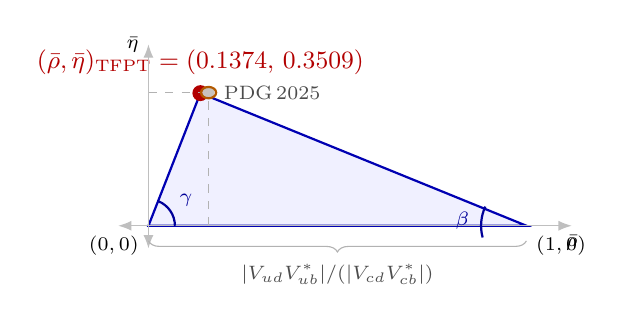
\begin{tikzpicture}[>=Latex, scale=4.8]
    \coordinate (O) at (0,0);
    \coordinate (B) at (1,0);
    \coordinate (A) at (0.1374,0.3509);

    \fill[blue!6] (O) -- (A) -- (B) -- cycle;
    \draw[thick, blue!70!black] (O) -- (B) -- (A) -- cycle;

    \fill[red!70!black] (A) circle (0.6pt);
    \node[above=3pt, font=\small\bfseries, red!70!black] at (A)
        {$(\bar\rho,\bar\eta)_{\mathrm{TFPT}}=(0.1374,\,0.3509)$};

    \draw[dashed, gray!60, thin] (0.1591,0) -- (0.1591,0.3523);
    \draw[dashed, gray!60, thin] (0,0.3523) -- (0.1591,0.3523);
    \fill[gray!70] (0.1591,0.3523) circle (0.45pt);
    \node[right=2pt, font=\scriptsize, gray!60!black] at (0.1591,0.3523)
        {PDG\,2025};

    \draw[thick, orange!70!black, fill=orange!12, fill opacity=0.4]
        (0.1591,0.3523) ellipse (0.020 and 0.015);

    \draw[<->, thin, gray!50] (-0.08,0) -- (1.12,0);
    \draw[<->, thin, gray!50] (0,-0.06) -- (0,0.48);
    \node[below, font=\scriptsize] at (1.12,0) {$\bar\rho$};
    \node[left, font=\scriptsize] at (0,0.48) {$\bar\eta$};

    \node[below left, font=\scriptsize] at (O) {$(0,0)$};
    \node[below right, font=\scriptsize] at (B) {$(1,0)$};

    \draw[decorate, decoration={brace, amplitude=4pt, mirror}, gray!60]
        (0,-0.04) -- (1,-0.04)
        node[midway, below=5pt, font=\scriptsize, gray!60!black]
        {$|V_{ud}V_{ub}^*|/(|V_{cd}V_{cb}^*|)$};

    \draw[blue!60!black, thick] (B) ++(155:0.12) arc (155:195:0.12);
    \node[font=\scriptsize, blue!60!black] at ($(B)+(175:0.17)$) {$\beta$};
    \draw[blue!60!black, thick] (O) ++(0:0.07) arc (0:69:0.07);
    \node[font=\scriptsize, blue!60!black] at ($(O)+(34:0.12)$) {$\gamma$};
\end{tikzpicture}
\caption{Unitarity triangle in the $(\bar\rho,\bar\eta)$ plane. The red dot marks
the exact TFPT apex from the full CKM matrix; the orange ellipse is an
illustrative $1\sigma$ region based on PDG\,2025 \cite{PDG2025} central values and
uncertainties. The TFPT apex uses the exact definition
$\bar\rho+i\bar\eta=-V_{ud}V_{ub}^*/(V_{cd}V_{cb}^*)$.}
\label{fig:unitarity-triangle}
\end{figure}


\section{Matching to short-distance amplitudes}
\label{sec:matching}

The matching map from the imported kernel and the sector data to the rare
kaon observables factorizes through the exact TFPT CKM matrix:
\begin{equation}
\label{eq:matching-map}
\mathcal M_{\mathrm{RK}}
:
\bigl(\text{TFPT kernel},\;\mathcal D_{\mathrm{RK}}\bigr)
\;\xrightarrow{\;\text{transport}\;}\;
(V_{\mathrm{CKM}})
\;\xrightarrow{\;\text{SD matching}\;}\;
\bigl(\BR(K^+),\,\BR(K_L)\bigr).
\end{equation}

\begin{definition}[Standard short-distance branching ratios]
\label{def:br-formulas}
We use the standard modern short-distance formulas \cite{BrodGorbahnStamou}:
\begin{equation}
\label{eq:br-kplus}
\BR(K^+\!\to\pi^+\nu\bar\nu)
=
\kappa_+\,(1+\Delta_{\mathrm{EM}})
\left[
\left(\frac{\im\lambda_t}{\lambda^5}\,X_t\right)^{\!2}
+
\left(
\frac{\re\lambda_c}{\lambda}\,(P_c+\delta P_{c,u})
+
\frac{\re\lambda_t}{\lambda^5}\,X_t
\right)^{\!2}
\right],
\end{equation}
\begin{equation}
\label{eq:br-kl}
\BR(K_L\to\pi^0\nu\bar\nu)
=
\kappa_L\,r_{\epsilon_K}
\left(\frac{\im\lambda_t}{\lambda^5}\,X_t\right)^{\!2},
\end{equation}
where $\lambda_t:=V_{ts}^*V_{td}$, $\lambda_c:=V_{cs}^*V_{cd}$,
$\lambda:=|V_{us}|=s_{12}$,
$X_t$ is the top-quark Inami--Lim function including NLO QCD and
electroweak corrections, $P_c$ is the charm contribution at NNLO QCD
and NLO EW, $\delta P_{c,u}$ is the long-distance charm--up
interference correction, and $r_{\epsilon_K}$ accounts for indirect
CP violation in the $K_L$ state.
\end{definition}

\begin{tcolorbox}[colback=gray!4, colframe=gray!60, breakable,
    title={\textbf{Short-distance input parameters}}, fonttitle=\bfseries]
\begin{itemize}[leftmargin=1.6em, itemsep=0.3em]
\item $X_t = 1.462\pm 0.017$ \quad (NLO QCD + NLO EW, at
      $m_t^{\mathrm{pole}}=\SI{172.6}{GeV}$, $M_W=\SI{80.36}{GeV}$);
\item $P_c = (0.2255/\lambda)^4\,(0.3604\pm 0.0087)$ \quad (NNLO QCD + NLO EW);
\item $\delta P_{c,u}=0.04\pm 0.02$ \quad (long-distance charm--up interference);
\item $\Delta_{\mathrm{EM}}=-0.003$ \quad (electromagnetic correction to $K^+$);
\item $\kappa_+=\num{5.173e-11}\,(\lambda/0.225)^8$,\;
      $\kappa_L=\num{2.231e-10}\,(\lambda/0.225)^8$;
\item $|\epsilon_K|=(\num{2.228}\pm\num{0.011})\times 10^{-3}$.
\end{itemize}
\end{tcolorbox}

At the present level of precision, the small indirect-CP-violation
correction to the neutral mode is included through \cite{BrodGorbahnStamou}
\begin{equation}
\label{eq:r-epsilon-K}
r_{\epsilon_K}
=
1
-\frac{\sqrt{2}\,|\epsilon_K|}
{1+P_c/(A^2 X_t)-\rho/\eta},
\qquad
\rho=\frac{\bar\rho}{1-\lambda^2/2},
\quad
\eta=\frac{\bar\eta}{1-\lambda^2/2}.
\end{equation}
On the TFPT branch, with $\bar\rho=0.1374$, $\bar\eta=0.3509$,
$A=0.8624$, $\lambda=0.22438$, this yields
\begin{equation}
\label{eq:r-epsilon-K-value}
r_{\epsilon_K}^{\mathrm{TFPT}}\approx 0.997.
\end{equation}

\begin{tcolorbox}[colback=blue!3, colframe=blue!50!black, breakable,
    title={\textbf{TFPT-fixed rare kaon prediction}}, fonttitle=\bfseries]
\begin{proposition}[TFPT-fixed CKM branching ratios with standard SD input]
\label{prop:br-prediction}
Insert the exact TFPT CKM products $\lambda_t$, $\lambda_c$ from
\Cref{eq:lambda-t-exact,eq:lambda-c-exact} into
\Cref{eq:br-kplus,eq:br-kl} with the short-distance parameters above.
TFPT fixes the CKM point without a flavor fit.
The short-distance functions $X_t$, $P_c$, $\delta P_{c,u}$, the
electromagnetic correction $\Delta_{\mathrm{EM}}$, and the hadronic
normalization constants $\kappa_\pm$ are standard external inputs.
The factor $r_{\epsilon_K}$ is derived from $|\epsilon_K|$ and the
TFPT CKM point via \Cref{eq:r-epsilon-K}.
The numerical evaluation yields
\begin{equation}
\label{eq:br-values}
\boxed{
\BR(K^+\!\to\pi^+\nu\bar\nu)
=
\num{9.40e-11},
\qquad
\BR(K_L\to\pi^0\nu\bar\nu)
=
\num{3.47e-11}.
}
\end{equation}
\end{proposition}
\end{tcolorbox}

\begin{proof}[Evaluation chain]
From \Cref{eq:lambda-t-exact,eq:lambda-c-exact} with
$\lambda=s_{12}=\num{0.22438}$:
\[
\frac{\im\lambda_t}{\lambda^5}
=
\frac{\num{1.522e-4}}{(0.22438)^5}
=
\num{0.2856},
\qquad
\frac{\re\lambda_t}{\lambda^5}
=
\frac{-\num{3.558e-4}}{(0.22438)^5}
=
\num{-0.6677},
\]
\[
\frac{\re\lambda_c}{\lambda}
=
\frac{-\num{0.2183}}{0.22438}
=
\num{-0.9729}.
\]
With $X_t=1.462$, $P_c=(0.2255/0.22438)^4\times 0.3604=\num{0.3625}$,
$\delta P_{c,u}=0.04$, $\Delta_{\mathrm{EM}}=-0.003$,
$\kappa_+=\num{5.173e-11}\times(0.22438/0.225)^8=\num{4.98e-11}$,
$\kappa_L=\num{2.231e-10}\times(0.22438/0.225)^8=\num{2.147e-10}$,
$r_{\epsilon_K}^{\mathrm{TFPT}}=0.997$:

\medskip
\noindent\textbf{Charged mode:}
\[
\BR(K^+)
=
\kappa_+'\times\bigl[
(\num{0.4175})^2
+
(\num{-1.3682})^2
\bigr]
=
\num{4.97e-11}\times\num{1.891}
=
\num{9.40e-11},
\]
where $\kappa_+'=\kappa_+(1+\Delta_{\mathrm{EM}})=\num{4.97e-11}$,
the CP-violating piece is $\im\lambda_t\,X_t/\lambda^5=\num{0.4175}$,
and the CP-conserving piece is
\[
\frac{\re\lambda_c}{\lambda}(P_c+\delta P_{c,u})
+\frac{\re\lambda_t}{\lambda^5}X_t
=
\num{-0.3917}-\num{0.9765}
=
\num{-1.3682}.
\]

\noindent\textbf{Neutral mode:}
\[
\BR(K_L)
=
\num{2.147e-10}\times 0.997
\times(0.2856\times 1.462)^2
=
\num{3.47e-11}.
\]
\end{proof}

\begin{remark}
The $K_L$ channel is purely CP violating and therefore proportional to
$(\im\lambda_t)^2$.
Since $\im\lambda_t\propto\bar\eta\propto\sin\delta_{\mathrm{CKM}}$,
the neutral-channel prediction is a direct test of the TFPT holonomy
phase $\delta_{\mathrm{CKM}}=\pi/3+3\lambda_C^2+O(\lambda_C^4)$.
The charged channel receives a sizeable charm admixture through
$P_c+\delta P_{c,u}$ and is therefore a less clean probe of the
CP phase alone, but a stronger test of the overall CKM norm.
\end{remark}


\subsection{Grossman--Nir correlation}

The model-independent Grossman--Nir (GN) bound provides a
constraint between the two channels that holds in any model
respecting isospin:
\begin{equation}
\label{eq:gn-bound}
\BR(K_L\to\pi^0\nu\bar\nu)
\;\le\;
4.3\;\BR(K^+\!\to\pi^+\nu\bar\nu).
\end{equation}
On the TFPT branch the ratio is
\begin{equation}
\label{eq:gn-ratio}
\frac{\BR(K_L)}{\BR(K^+)}
=
\frac{\num{3.47e-11}}{\num{9.40e-11}}
=
0.369,
\end{equation}
safely within the isospin corridor $(\le 4.3)$.

\begin{figure}[t]
\centering
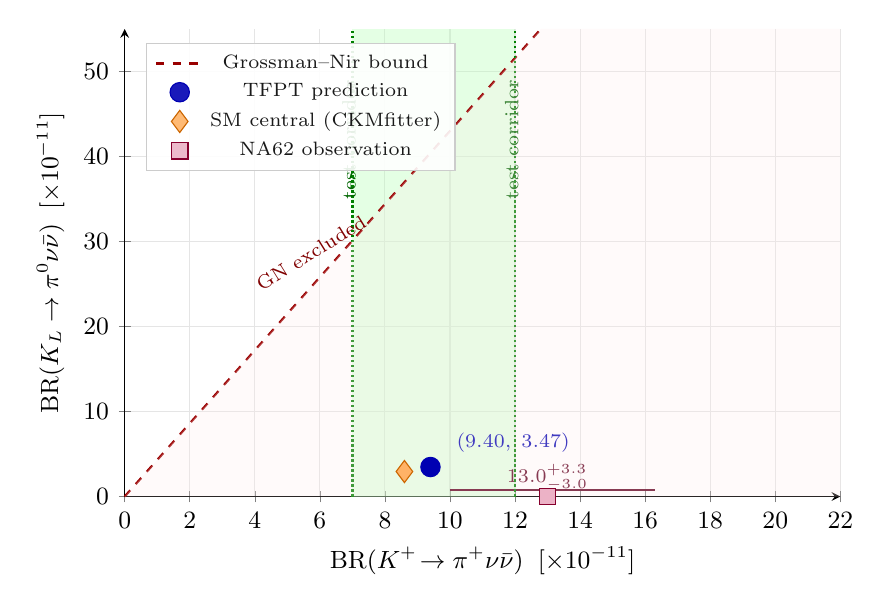
\begin{tikzpicture}
\begin{axis}[
    width=0.88\linewidth,
    height=0.62\linewidth,
    xlabel={$\BR(K^+\!\to\pi^+\nu\bar\nu)\;\;[\times 10^{-11}]$},
    ylabel={$\BR(K_L\to\pi^0\nu\bar\nu)\;\;[\times 10^{-11}]$},
    xmin=0, xmax=22,
    ymin=0, ymax=55,
    grid=major,
    grid style={gray!20},
    axis lines=left,
    tick label style={font=\small},
    label style={font=\small},
    legend style={font=\scriptsize, at={(0.03,0.97)}, anchor=north west,
        draw=gray!40, fill=white, fill opacity=0.9},
    clip=false,
]

\addplot[domain=0:12.8, samples=80, thick, red!60!black, dashed,
    name path=gn] {4.3*x};
\addlegendentry{Grossman--Nir bound}

\addplot[only marks, mark=*, mark size=3.5pt, blue!70!black, fill=blue!70!black]
    coordinates {(9.40, 3.47)};
\addlegendentry{TFPT prediction}

\addplot[only marks, mark=diamond*, mark size=4pt, orange!80!black,
    fill=orange!60!white]
    coordinates {(8.60, 2.94)};
\addlegendentry{SM central (CKMfitter)}

\addplot[only marks, mark=square*, mark size=3pt, purple!70!black,
    fill=purple!30!white]
    coordinates {(13.0, 0)};
\addlegendentry{NA62 observation}
\draw[purple!50!black, thick] (axis cs:10.0,0.8) -- (axis cs:16.3,0.8);
\node[font=\scriptsize, purple!50!black] at (axis cs:13.0,2.2) {$13.0^{+3.3}_{-3.0}$};

\addplot[name path=killL, draw=none] coordinates {(7,0) (7,55)};
\addplot[name path=killR, draw=none] coordinates {(12,0) (12,55)};
\addplot[green!30, opacity=0.35] fill between[of=killL and killR];

\draw[green!50!black, thick, densely dotted] (axis cs:7,0) -- (axis cs:7,55);
\draw[green!50!black, thick, densely dotted] (axis cs:12,0) -- (axis cs:12,55);

\node[font=\scriptsize, green!40!black, rotate=90, anchor=south]
    at (axis cs:7.4,42) {test corridor};
\node[font=\scriptsize, green!40!black, rotate=90, anchor=south]
    at (axis cs:12.4,42) {test corridor};

\node[font=\scriptsize, blue!70!black, anchor=south west]
    at (axis cs:9.9,4.0) {$(9.40,\;3.47)$};

\fill[red!8, opacity=0.25] (axis cs:0,0) -- (axis cs:12.8,55.04) --
    (axis cs:22,55.04) -- (axis cs:22,0) -- cycle;
\node[font=\scriptsize, red!50!black, rotate=32, anchor=south]
    at (axis cs:6.0,27) {GN excluded};

\end{axis}
\end{tikzpicture}
\caption{Grossman--Nir plane for $K\to\pi\nu\bar\nu$. The dashed red line is
the model-independent isospin bound $\BR(K_L)\le4.3\,\BR(K^+)$; the region
above it is excluded. The blue dot marks the TFPT prediction; the orange
diamond shows the SM central value from CKMfitter. The purple square shows
the NA62 combined measurement $(13.0^{+3.3}_{-3.0})\times10^{-11}$
(charged channel only; the $K_L$ measurement has not yet reached SM sensitivity).
The green corridor $[7,12]\times10^{-11}$ is the operational TFPT test window
for the charged channel; it is not a formal confidence interval but an
approximate consistency band around the central prediction.}
\label{fig:gn-plane}
\end{figure}

Any future measurement placing the experimental ratio above $4.3$
would signal physics outside the SM operator basis and would
simultaneously invalidate the TFPT matching ansatz for this sector.
The predicted point in the $(K^+,K_L)$ plane is shown as a fixed target
in \Cref{fig:gn-plane}.


\section{Benchmark ledger}
\label{sec:benchmarks}

\begin{table}[ht]
\centering
\footnotesize
\begin{tabularx}{\linewidth}{@{}>{\raggedright\arraybackslash}p{0.17\linewidth}>{\raggedright\arraybackslash}Y>{\raggedright\arraybackslash}p{0.16\linewidth}>{\raggedright\arraybackslash}p{0.17\linewidth}>{\centering\arraybackslash}p{0.11\linewidth}@{}}
\toprule
Observable & TFPT value & Imported input & Sector input & Status \\
\midrule
$\BR(K^+\!\to\pi^+\nu\bar\nu)$
  & $\num{9.40e-11}$
  & $\phiz,\lambda_C,\delta_{\mathrm{CKM}}$
  & $X_t$, $P_c$, $\delta P_{c,u}$, $\Delta_{\mathrm{EM}}$, $\kappa_+$
  & prediction \\[6pt]
$\BR(K_L\to\pi^0\nu\bar\nu)$
  & $\num{3.47e-11}$
  & $\phiz,\lambda_C,\delta_{\mathrm{CKM}}$
  & $X_t$, $\kappa_L$, $|\epsilon_K|$
  & prediction \\[6pt]
$\BR(K_L)/\BR(K^+)$
  & $0.369$
  & CKM point
  & isospin ($\kappa_L/\kappa_+$)
  & GN test \\[6pt]
$\delta_{\mathrm{CKM}}$
  & $\num{1.198}$ rad
  & holonomy phase
  & ---
  & anchor \\[6pt]
$\lambda_C$
  & $\num{0.22438}$
  & $\sqrt{\phiz(1-\phiz)}$
  & ---
  & anchor \\
\bottomrule
\end{tabularx}
\caption{Benchmark ledger for the rare kaon note. The first two rows
are the primary predictions. The third is a derived GN-plane test.
The last two rows record the kernel anchors whose values propagate
into the branching ratios.}
\label{tab:benchmark-ledger}
\end{table}

\begin{table}[ht]
\centering
\small
\begin{tabularx}{\linewidth}{@{}>{\raggedright\arraybackslash}p{0.14\linewidth}>{\centering\arraybackslash}p{0.12\linewidth}>{\centering\arraybackslash}p{0.14\linewidth}>{\raggedright\arraybackslash}Y>{\centering\arraybackslash}p{0.09\linewidth}@{}}
\toprule
Parameter & TFPT & PDG\,'25 & Derivation chain & Pull \\
\midrule
$\lambda$ & $\num{0.22438}$ & $0.22501(68)$ & $\sqrt{\phiz(1-\phiz)}$ & $0.9\sigma$ \\
$A$ & $\num{0.8624}$ & $0.826^{+0.016}_{-0.015}$ & $\phiz/[\lambda^2(1+\lambda)]$ & $2.3\sigma$ \\
$\bar\rho$ & $\num{0.1374}$ & $0.1591(94)$ & exact $-V_{ud}V_{ub}^*/(V_{cd}V_{cb}^*)$ & $2.3\sigma$ \\
$\bar\eta$ & $\num{0.3509}$ & $0.3523(73)$ & exact $-V_{ud}V_{ub}^*/(V_{cd}V_{cb}^*)$ & $0.2\sigma$ \\
$\delta$ & $\num{1.198}$ rad & $1.147(26)$ rad & holonomy phase & $2.0\sigma$ \\
\bottomrule
\end{tabularx}
\caption{Exact TFPT CKM point versus the PDG\,2025 \cite{PDG2025} global fit.
The pulls for $A$, $\bar\rho$, and $\delta$ are at the $2\sigma$ level,
indicating genuine tension that the rare kaon measurements can resolve.}
\label{tab:wolfenstein}
\end{table}

The two branching-ratio rows depend on the imported CKM point
(from the kernel seed and the transport grammar) and on standard
electroweak loop functions (sector-specific, but not TFPT specific).
Every TFPT-specific content enters through $\lambda_C$,
$\delta_{\mathrm{CKM}}$, and the exact CKM matrix built from them.
The factor $r_{\epsilon_K}$ is not an independent external constant but
is derived from $|\epsilon_K|$ and the TFPT CKM point.


\section{Sensitivity anatomy}
\label{sec:sensitivity}

The charged and neutral branching ratios respond differently to the kernel
parameters. Schematically:
\begin{equation}
\label{eq:sensitivity}
\frac{\partial\ln\BR(K_L)}{\partial\ln\bar\eta}\;=\;2,
\qquad
\frac{\partial\ln\BR(K^+)}{\partial\ln\bar\eta}\;\approx\;1.4,
\end{equation}
so the neutral channel is the sharper probe of $\bar\eta$ and hence of
$\sin\delta_{\mathrm{CKM}}$.

Because $\delta_{\mathrm{CKM}}$ on the TFPT branch has the structure
$\pi/3+3\lambda_C^2+\cdots$, a tension in $\BR(K_L)$ would
propagate directly into either the holonomy base phase $\pi/3$
or the transport area correction $3\lambda_C^2$.
Conversely, the charged channel has a sizeable charm-sector
admixture through $P_c+\delta P_{c,u}$ and is therefore a less clean
probe of the CP phase alone, but a stronger test of the overall CKM norm.

The $2\sigma$ tensions in $A$, $\bar\rho$, and $\delta$ visible in
\Cref{tab:wolfenstein} are not fatal but make the rare kaon corridor a
genuinely discriminating test: NA62 precision data will push the comparison
from ``consistent'' to ``confirmed or excluded''.


\section{Falsification matrix}
\label{sec:falsification}

\begin{figure}[t]
\centering
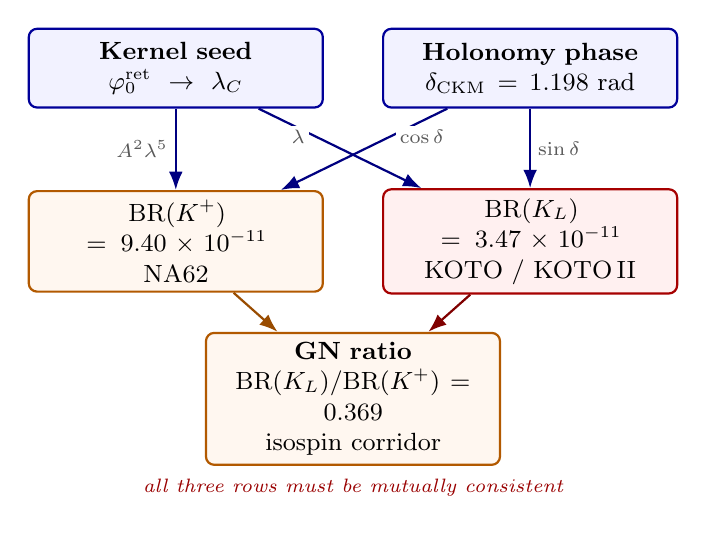
\begin{tikzpicture}[
    >=Latex,
    kill/.style={draw=red!65!black, thick, rounded corners=3pt,
        fill=red!6, align=center, text width=3.5cm, minimum height=1.0cm,
        font=\small},
    kernelnode/.style={draw=blue!60!black, thick, rounded corners=3pt,
        fill=blue!5, align=center, text width=3.5cm, minimum height=1.0cm,
        font=\small},
    pressure/.style={draw=orange!70!black, thick, rounded corners=3pt,
        fill=orange!6, align=center, text width=3.5cm, minimum height=1.0cm,
        font=\small},
    arrlabel/.style={font=\scriptsize, fill=white, inner sep=1.5pt,
        text=gray!70!black},
]
\node[kernelnode] (seed) at (0,0) {\textbf{Kernel seed}\\$\phiz\to\lambda_C$};
\node[kernelnode] (phase) at (4.5,0) {\textbf{Holonomy phase}\\$\delta_{\mathrm{CKM}}=1.198$ rad};

\node[pressure] (kplus) at (0,-2.2)
    {\textbf{$\BR(K^+)$}\\$=9.40\times10^{-11}$\\NA62};
\node[kill] (kl) at (4.5,-2.2)
    {\textbf{$\BR(K_L)$}\\$=3.47\times10^{-11}$\\KOTO / KOTO\,II};

\node[pressure] (gn) at (2.25,-4.2)
    {\textbf{GN ratio}\\$\BR(K_L)/\BR(K^+)=0.369$\\isospin corridor};

\draw[->, thick, blue!50!black] (seed) -- (kplus)
    node[arrlabel, midway, left=1pt]{$A^2\lambda^5$};
\draw[->, thick, blue!50!black] (seed) -- (kl)
    node[arrlabel, midway, left=2pt, pos=0.35]{$\lambda$};
\draw[->, thick, blue!50!black] (phase) -- (kl)
    node[arrlabel, midway, right=1pt]{$\sin\delta$};
\draw[->, thick, blue!50!black] (phase) -- (kplus)
    node[arrlabel, midway, right=2pt, pos=0.35]{$\cos\delta$};

\draw[->, thick, orange!60!black] (kplus) -- (gn);
\draw[->, thick, red!50!black] (kl) -- (gn);

\node[font=\scriptsize\itshape, text=red!60!black, anchor=north]
    at (2.25,-5.1) {all three rows must be mutually consistent};
\end{tikzpicture}
\caption{Falsification dependency graph. Blue anchors feed both branching
ratio predictions. The GN ratio provides a correlated cross-check.
A failure at any node propagates upward into the TFPT flavor bridge.}
\label{fig:falsification-graph}
\end{figure}

\begin{table}[ht]
\centering
\small
\begin{tabularx}{\linewidth}{@{}>{\raggedright\arraybackslash}p{0.21\linewidth}>{\raggedright\arraybackslash}p{0.23\linewidth}>{\centering\arraybackslash}p{0.13\linewidth}>{\raggedright\arraybackslash}Y@{}}
\toprule
Test & Kill criterion & Depends on & Consequence if failed \\
\midrule
$\BR(K^+)$ outside $[7,12]\times 10^{-11}$
  & stable NA62 result
  & CKM point
  & breaks the full TFPT flavor bridge \\[4pt]
$\BR(K_L)$ incompatible with TFPT point
  & KOTO / KOTO\,II result
  & $\im\lambda_t$ (phase)
  & breaks the holonomy-phase prediction \\[4pt]
GN ratio $>4.3$
  & combined $K^+/K_L$ measurement
  & isospin
  & new-physics operator beyond SM basis \\[4pt]
$\delta_{\mathrm{CKM}}$ excluded at ${\ge}3\sigma$
  & global unitarity-triangle fit
  & holonomy grammar
  & breaks the $\mathbb Z_6$ transport base phase \\[4pt]
$\lambda_C$ shifts by $>3\sigma$
  & improved $|V_{us}|$ determination
  & kernel seed $\phiz$
  & breaks the seed-chain anchor \\
\bottomrule
\end{tabularx}
\caption{Falsification matrix. The corridor $[7,12]\times10^{-11}$
is an operational test window around the central $K^+$ prediction,
not a formal confidence interval.
The last two rows are upstream kernel anchors whose failure would
propagate into the rare kaon prediction.}
\label{tab:falsification}
\end{table}

\begin{itemize}[leftmargin=1.6em, itemsep=0.3em]
\item The sharpest single kill test is a stable NA62 measurement of
$\BR(K^+)$ outside $[7,12]\times 10^{-11}$. This operational corridor
is chosen to bracket the TFPT central value including the dominant
short-distance and CKM parametric uncertainties; it is not a formal
$n\sigma$ band.
The current NA62 observation $(13.0^{+3.3}_{-3.0})\times 10^{-11}$
is consistent with the TFPT value at $1\sigma$.
\item The cleanest CP-phase test is the $K_L$ channel: because
$\BR(K_L)\propto(\im\lambda_t)^2\propto\bar\eta^2$, any
disagreement between a future KOTO\,II measurement and
$\num{3.47e-11}$ directly constrains $\sin\delta_{\mathrm{CKM}}$.
\item A GN-violating measurement ($\BR(K_L)/\BR(K^+)>4.3$) would not
kill TFPT specifically but would signal new-physics operators outside
the SM basis used in the matching.
\item The upstream kernel anchors $\lambda_C$ and $\delta_{\mathrm{CKM}}$
are independently testable: $\lambda_C$ through precision $|V_{us}|$
measurements, and $\delta_{\mathrm{CKM}}$ through the global CKM fit.
The $\delta$ tension is currently at $2.0\sigma$ (\Cref{tab:wolfenstein}).
\end{itemize}


\section{Experimental landscape}
\label{sec:experiment}

The NA62 experiment at CERN has observed the decay
$K^+\to\pi^+\nu\bar\nu$ with a combined (2016--2022)
branching ratio measurement of \cite{NA62obs}
\[
\BR(K^+\to\pi^+\nu\bar\nu)
=
(13.0^{+3.3}_{-3.0})\times 10^{-11},
\]
based on 51 signal candidates at a significance exceeding $5\sigma$.
The TFPT prediction of $\num{9.40e-11}$ is consistent with this
measurement at the $1\sigma$ level and will be tested with improving
precision as NA62 continues data-taking.

The $K_L\to\pi^0\nu\bar\nu$ channel is pursued by the KOTO experiment
at J-PARC, which currently sets the direct limit \cite{KOTO}
\[
\BR(K_L\to\pi^0\nu\bar\nu)<\num{2.2e-9}
\quad\text{(90\% C.L.)},
\]
still more than an order of magnitude above the SM and TFPT predictions.
The planned successor KOTO\,II aims to reach SM sensitivity, at which
point the TFPT prediction of $\num{3.47e-11}$ becomes a genuine
pressure test.

The combined $(K^+,K_L)$ measurement in the Grossman--Nir plane
provides the most powerful correlated test: the TFPT point
$(\num{9.40e-11},\,\num{3.47e-11})$ is a fixed target that can be
confronted with the experimental ellipse as both channels are measured.


\section{Conclusion}
\label{sec:conclusion}

\begin{tcolorbox}[colback=gray!4, colframe=gray!60, breakable,
    title={\textbf{Summary}}, fonttitle=\bfseries]
\begin{enumerate}[label=\arabic*., leftmargin=1.6em, itemsep=0.3em]
\item The TFPT minimal kernel, through the retained seed $\phiz$ and the
$\mathbb Z_6$ family transport grammar, fixes the full CKM matrix---including
the exact apex coordinates $(\bar\rho,\bar\eta)=(0.1374,\,0.3509)$---without
fitting to flavor data.
\item The exact CKM point, combined with standard modern short-distance input
($X_t$, $P_c$, $\delta P_{c,u}$, $\Delta_{\mathrm{EM}}$) and the
derived factor $r_{\epsilon_K}^{\mathrm{TFPT}}=0.997$,
yields TFPT-fixed branching ratios:
$\BR(K^+)=\num{9.40e-11}$ and $\BR(K_L)=\num{3.47e-11}$.
\item The sharpest falsification handle is a stable NA62 measurement of
$\BR(K^+)$ outside the operational test corridor $[7,12]\times 10^{-11}$,
or a KOTO\,II result for $\BR(K_L)$ incompatible with the predicted
GN-plane point, either of which would break the TFPT flavor bridge.
The current NA62 observation $(13.0^{+3.3}_{-3.0})\times 10^{-11}$
is consistent at $1\sigma$.
\end{enumerate}
\end{tcolorbox}


\begin{thebibliography}{9}

\bibitem{TFPT}
S.~Hamann and A.~Rizzo,
\textit{TFPT: A carrier-first compiler for the Standard Model and beyond},
(2026).

\bibitem{BrodGorbahnStamou}
J.~Brod, M.~Gorbahn, and E.~Stamou,
Updated Standard Model prediction for $K\to\pi\nu\bar\nu$ and
$\epsilon_K$,
\textit{PoS} \textbf{BEAUTY2020} (2021) 056;
see also \textit{Phys.\ Rev.\ D} \textbf{105} (2022) 014036.

\bibitem{BurasRareKaons}
A.~J.~Buras, D.~Buttazzo, J.~Girrbach-Noe, and R.~Knegjens,
$K^+\to\pi^+\nu\bar\nu$ and $K_L\to\pi^0\nu\bar\nu$ in the Standard
Model: status and perspectives,
\textit{JHEP} \textbf{11} (2015) 033.

\bibitem{GrossmanNir}
Y.~Grossman and Y.~Nir,
$K_L\to\pi^0\nu\bar\nu$ beyond the Standard Model,
\textit{Phys.\ Lett.\ B} \textbf{398} (1997) 163.

\bibitem{NA62obs}
NA62 Collaboration,
Observation of the decay $K^+\to\pi^+\nu\bar\nu$,
CERN-EP-2024-252 (2024).

\bibitem{KOTO}
KOTO Collaboration,
Search for $K_L\to\pi^0\nu\bar\nu$ and
$K_L\to\pi^0 X^0$ decays at the J-PARC KOTO experiment,
\textit{Phys.\ Rev.\ Lett.} \textbf{126} (2021) 121801.

\bibitem{InamiLim}
T.~Inami and C.~S.~Lim,
Effects of superheavy quarks and leptons in low-energy weak processes
$K_L\to\mu\bar\mu$, $K^+\to\pi^+\nu\bar\nu$ and $K^0\leftrightarrow\bar K^0$,
\textit{Prog.\ Theor.\ Phys.} \textbf{65} (1981) 297.

\bibitem{PDG2025}
S.~Navas et al.\ (Particle Data Group),
\textit{Review of Particle Physics},
\textit{Phys.\ Rev.\ D} \textbf{110} (2024) 030001, updated 2025.

\end{thebibliography}

\end{document}
